\documentclass{article}

\usepackage{helvet}
\usepackage{pgfplotstable}
\usepackage{pdflscape}
\usepackage{graphicx}
\usepackage{makecell}
\usepackage{booktabs} 
\usepackage{rotating}
\usepackage{newclude}
\usepackage{color}
\usepackage[top=3cm, bottom=4cm, left=3.2cm, right=3.2cm]{geometry}
\usepackage{url}
\usepackage{natbib}
\usepackage{hyperref}
\usepackage{fancyhdr}
\usepackage{pdfpages}
\usepackage{floatpag}
\usepackage{caption}
\usepackage{longtable}
\usepackage{colortbl}
%\floatpagestyle{empty}
\usepackage{amssymb,amsmath,amsthm}
\usepackage[T1]{fontenc}
\usepackage{xcolor,colortbl}
\usepackage{tabularx}
\usepackage{multirow}
\usepackage{textcomp}
%\usepackage{draftwatermark}
\usepackage{listings}
\lstset{backgroundcolor=\color{lightgray!20}, basicstyle={\ttfamily}}

%\SetWatermarkText{For use at GMI only}
%\SetWatermarkColor[gray]{0.9}
%\SetWatermarkFontSize{2cm}

\pagestyle{fancy}
\fancyfoot[C]{MethylScore -- Manual}
\fancyhead[LO,LE]{\rightmark}
\fancyhead[RO,RE]{\thepage}
\renewcommand*\familydefault{\sfdefault}

\renewcommand{\thesection}{}
\renewcommand{\thesubsection}{\#\arabic{section}.\arabic{subsection}}
\renewcommand{\labelitemi}{$\blacktriangleright$}
\renewcommand{\labelitemii}{$\bullet$}

\captionsetup[table]{aboveskip=0pt}
\captionsetup[table]{belowskip=10pt}

\newcolumntype{N}{>{\global\let\currentrowstyle\relax}l}
\newcolumntype{B}{>{{\global\let\currentrowstyle\relax}\bfseries}l}
%\newcolumntype{R}{>{\currentrowstyle}r}
\newcolumntype{I}{>{{\currentrowstyle}\itshape \bfseries} r}
\newcommand{\rowstyle}[1]{\gdef\currentrowstyle{#1}%
	#1\ignorespaces
}
% for longtables:
\newcolumntype{R}[1]{>{\raggedleft\arraybackslash}p{#1}}

\pgfplotstableset{string type,col sep=comma,fixed, trim cells=true,
every head row/.style={before row=\toprule,after row=\midrule},
every last row/.style={after row=\bottomrule}}

\setlength{\parskip}{1mm}

\begin{document}

%cover page(s) separately 
\include*{coverpage}

\newpage

\tableofcontents

\newpage


This document describes the strategy and usage of MethylScore, a pipeline to call differential methylation between samples using next-generation sequencing. 
%Moreover, this text outlines the improvements over the publicly available DMR detection strategy of \cite{Hagmann2015}.

\section{MethylScore strategy}

The pipeline consists of several modules that can be run as a whole or one by one. The overall workflow and the used external tools with their versions are outlined in Figure \ref{fig:MSpipeline}.\\

In brief, the pipeline starts from mapping files of each sample or of each technical replicate. Mapping files are expected to be in bam format, produced by the bisulfite read mapping tool bwa-meth\footnote{\href{https://github.com/brentp/bwa-meth/archive/master.zip}{https://github.com/brentp/bwa-meth/archive/master.zip} (last accessed June 2017)} [\cite{bwa_meth}]. 

First, the mapping files of technical replicates are merged, each sample's mappings are de-duplicated using picardtools, then split by chromosome, and for each sample and chromosome, the numbers of methylated/unmethylated reads per position (pileup information) are retrieved using the tool MethylExtract.
The pileup information from all analyzed samples is summarized in a so-called genome matrix that is generated per sample and chromosome in parallel.

The global genome matrix serves as input for the detection of methylated regions per sample and the conversion to an igv file that can be used to visualize methylation information in the  \href{http://software.broadinstitute.org/software/igv/}{Integrative Genomics Viewer (IGV)}. Methylated regions (MRs) are determined by a two-state Hidden Markov Model (HMM)-based method that learns different methylation level distributions for an unmethylated and a methylated state from whole genome data (described in section \ref{MRs}).
%fits beta binomial distributions from whole genome data for an unmethylated and a methylated state. Thus, the HMM models different methylation level distributions, either from unmethylated or methylated regions. The most likely path through the two states along the genome directly provides methylated regions for each sample. 
%\footnote{For detailed information, refer to \cite{Hagmann2015}.}. 
%TODO For this step, data from biological samples are merged. However, the subsequent calling of differentially methylated regions (DMRs) takes the separate replicates into account.

Finally, to obtain significant differences in methylation on a regional scale between different samples, MethylScore, in short, clusters samples by methylation levels and statistically tests the group's methylation distributions for significant differences (described in section \ref{DMRs}).
%A precise description and its improvements over the method it is based on \cite{Hagmann2015} will be given in the next section.

\begin{figure}[p]
	\centering
	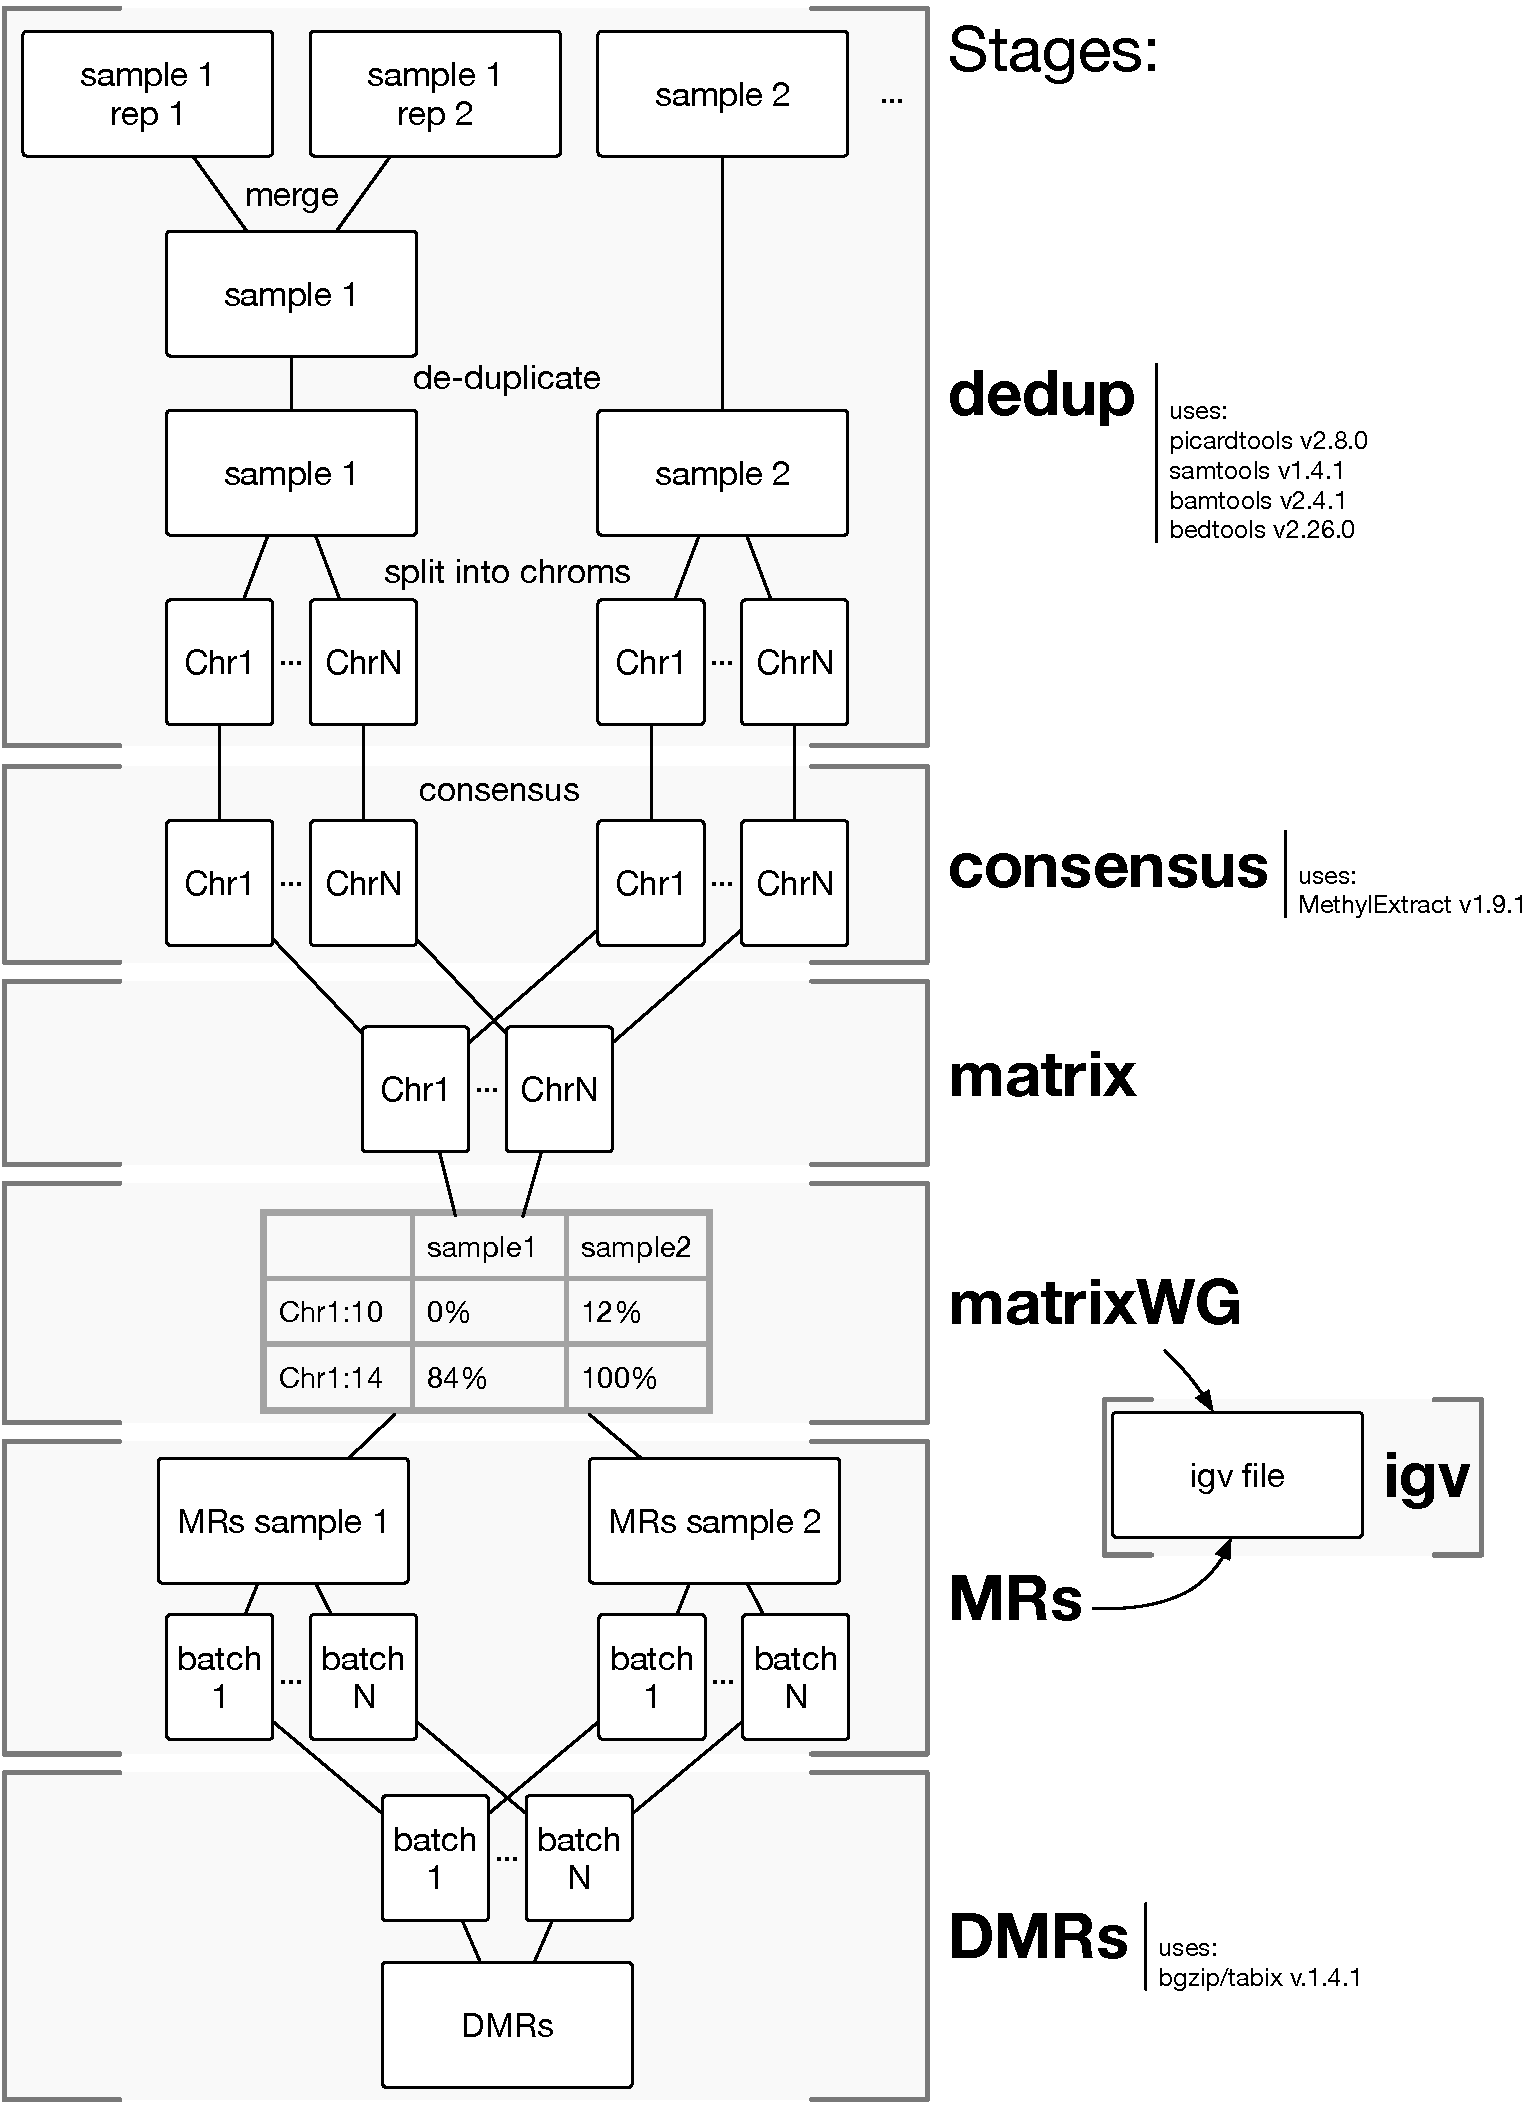
\includegraphics[width=.95\linewidth]{graphics/workflow.pdf}
	\caption[MethylScore analysis pipeline.]{MethylScore analysis pipeline. An example with two samples is shown, where sample 1 has two technical replicates (rep1, rep2). Horizontally arranged boxes represent tasks that can be run in parallel.}
	\label{fig:MSpipeline}
\end{figure}


\subsection{MR calling strategy}
\label{MRs}

MR calling is performed by applying a Hidden Markov Model that fits context-specific beta binomial distributions from whole genome data for an unmethylated and a methylated state. Given the trained model, sites are probabilistically classified into the most likely state via Posterior Decoding (default) or Viterbi's algorithm. The basic implementation was adapted from \cite{Molaro2011}.

\subsubsection*{Desert size parameter}
\label{desertsize}
The advantage of using an HMM is that it takes the directly preceding state into account. Chromosomes are 'natural' split points where the HMM decoding starts over again without previous state information. The HMM implementation described here has additional split points defined by a maximum genomic distance between adjacent covered cytosines. Regions of absent read coverage or cytosines are referred to as 'deserts' in the original implementation. In practice, it means that an MR cannot span a region without methylation information of the size of a desert (MethylScore parameter DESERT\_SIZE, default: 100\,bp).

\subsubsection*{Post-processing parameters}
\label{permutation_test}
Since consecutive sites in methylated state ("high methylation regions") can be very short, there are two alternative ways to finally define MRs:
\begin{enumerate}
	\item Permutation test: all covered cytosines are randomly shuffled and 'random' high methylation regions are called. High methylation regions are scored by the sum of the contained methylation rates. The scores of the 'real' high methylation regions are tested against the 'random' score distribution to calculate p-values. After FDR calculation, high methylation regions with an FDR of 0.01 (default) are defined as MRs.\\
	This strategy proved reasonable on whole-genome libraries and for species where most genome space is unmethylated (e.g. plants from the Arabidopsis genus and rice). %However, it was noted before that regions of low methylation density like gene body methylation have reduced MR calls compared to other methods that are based on clustering single sites\cite{Hagmann2015}.
	This strategy is followed if the MethylScore parameter MR\_MIN\_C is set to 0.
	\item Minimum number of cytosines: high methylation regions containing a minimum number of covered cytosines are defined as MRs.\\
	This simple length filter proves useful for methylation-enriched libraries or for species with a high fraction of methylated sequence, when a random shuffling of the genome already produces regions of moderate to high methylation density by chance. Then, moderately dense regions will be discarded by the permutation test. This second strategy remedies the described disadvantage of the permutation test and is chosen if the MethylScore parameter MR\_MIN\_C is set to a positive value.
\end{enumerate}

Besides an MR length filter as just described above, there are two additional post-processing filters to facilitate a biologically meaningful interpretation. Nearby MRs within a certain base pair distance can be merged into one region (MethylScore parameter MERGE\_DIST, default: 30\,bp, turned off: 0\,bp), and lowly methylated positions can be trimmed off the ends of MRs (MethylScore parameter TRIM\_METHRATE, default: sites below 10\,\% methylation rate are trimmed off, turned off: 0\,\%).


\subsection{DMR calling strategy}
\label{DMRs}

For calling DMRs, MethylScore focuses on the unified methylated genome space determined by the sample-specific MRs. To reduce complexity and ease the computation of a large number of samples, MethylScore follows a more coarse-grained, population-scale view compared to previous approaches [\cite{Hagmann2015}] in mainly two aspects:
\begin{itemize}
	\item Rather than testing a large set of candidate DMRs, generated by all combinations of individual MR start and end coordinates as the attempt to find the 'natural' borders of DMRs, MethylScore considers the MR distribution of the whole population of samples. Candidate DMRs are delimited by drastic, abrupt changes in the MR frequency across all samples. The underlying assumption is that frequent changes in methylation pattern among samples are more likely 'natural' borders of DMRs.
	\item Rather than performing all pairwise sample comparisons on each candidate DMR, MethylScore employs a routine clustering method to assign samples into groups and solely tests groups against each other for differential methylation.
\end{itemize}


\subsubsection*{Finding candidate DMRs}
\label{segments}

For each position at which the MR frequency changes (i.e. at all MR start and end positions), a candidate DMR is defined by the following rules (illustrated in Figure \ref{fig:segments}):

\begin{itemize}
	\item a new region is started if the MR frequency at the actual position changes by more than a user-defined percentage of the number of all samples (MethylScore parameter \mbox{MR\_FREQ\_CHANGE}) compared to the position before, or -- to account for gradual small-step changes -- compared to a position certain base pairs upstream (MethylScore parameter MR\_FREQ\_DISTANCE, default: 30\,bp).
	\item segments need to contain a minimum number of C's covered by a minimum read coverage in at least one sample (MethylScore parameters DMR\_MIN\_C and DMR\_MIN\_COV, default: 10 and 3x, respectively).
\end{itemize}

This represents roughly a clustering of the methylated genome space into major MR frequency classes of a sample population.
Longer segments could optionally be split into smaller ones using a sliding window approach.

\begin{figure}[h]
	\centering
	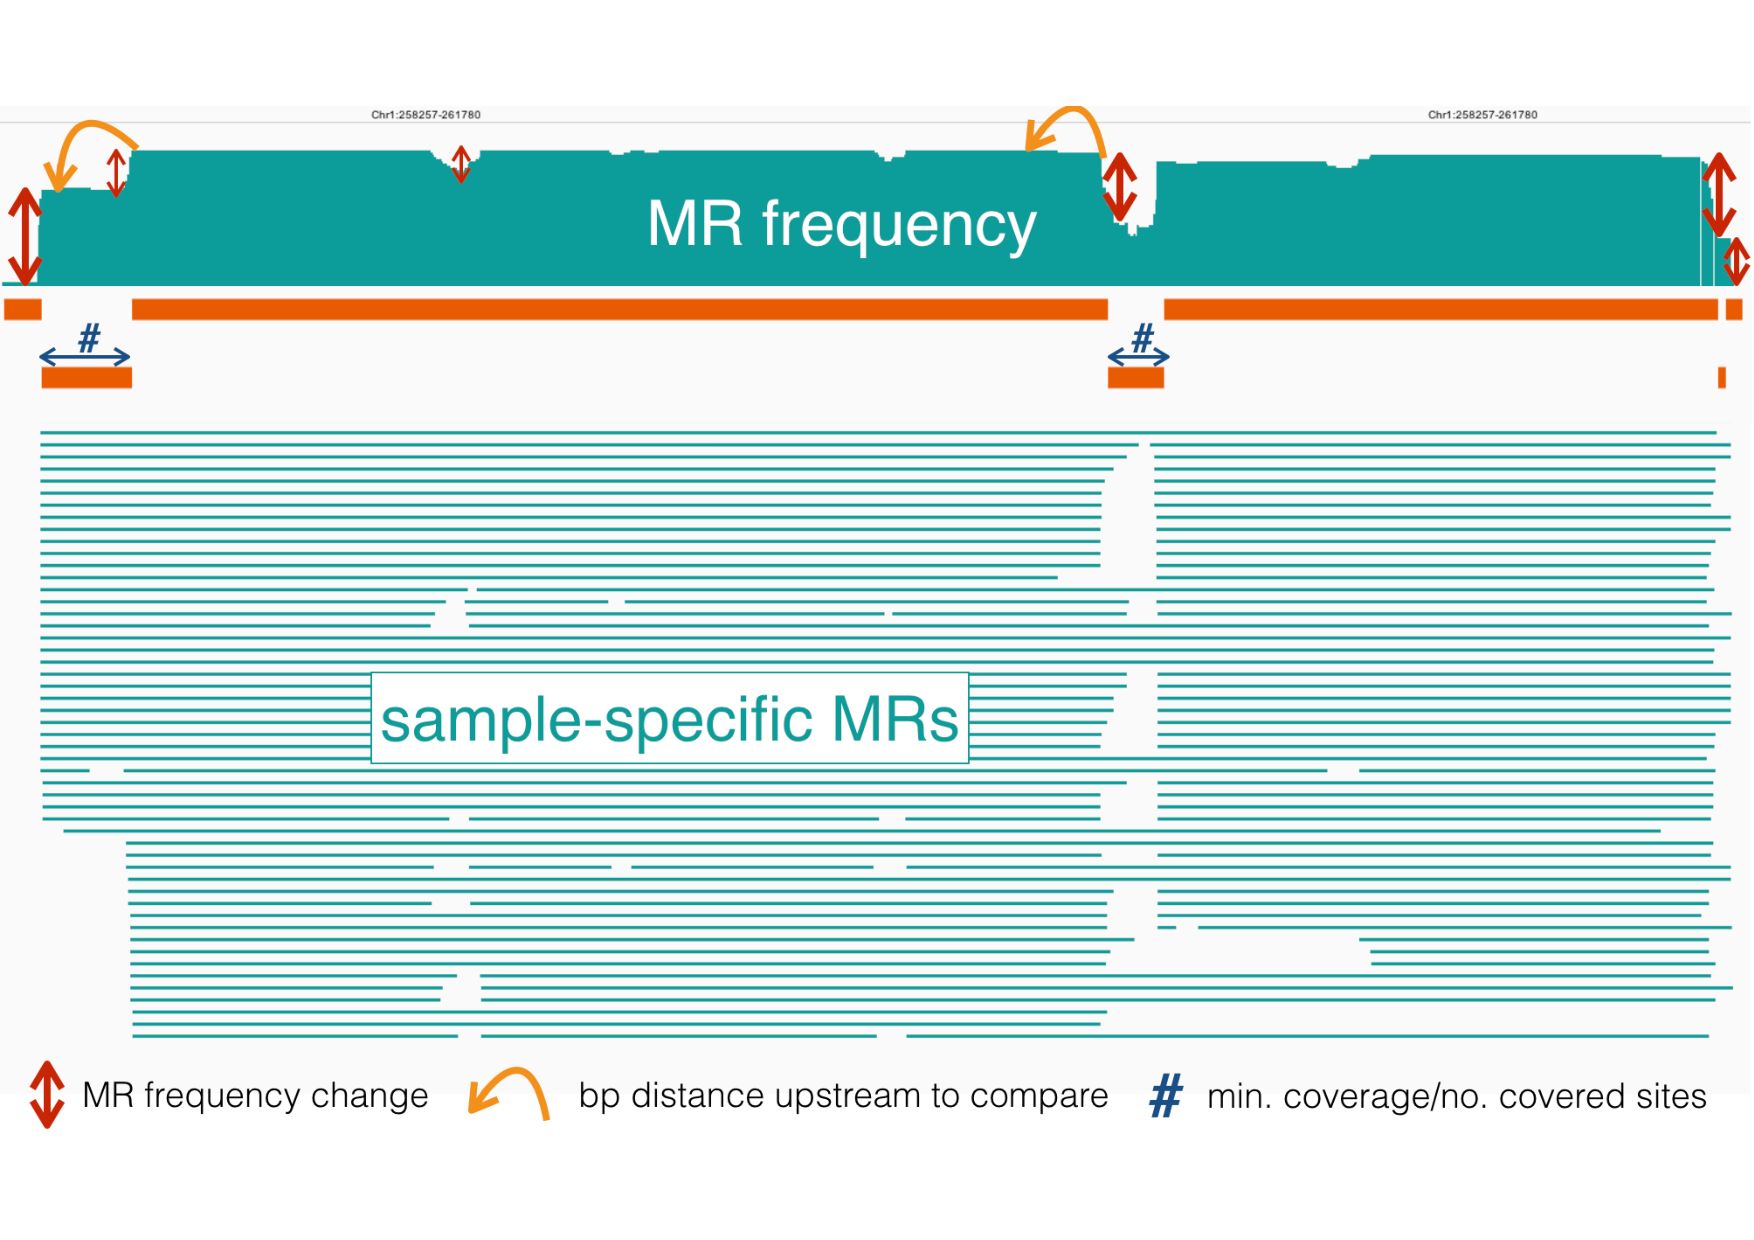
\includegraphics[width=0.9\linewidth]{graphics/segments.pdf}
	\caption[Determining candidate DMRs.]{Determining candidate DMRs. The top panel shows an MR frequency barplot along the genome, summarizing the counts of all sample-specific MRs (the MRs are displayed as horizontal petrol-colored lines in the middle). Three parameters specify the borders of candidate DMRs (orange horizontal bars): 1. the degree of MR frequency changes along the genome (marked by red vertical arrows), 2. the upstream distance to which MR frequency is compared to (marked by orange-colored bent arrows), and 3. a minimum number and coverage of cytosines (blue arrows indicating the length of candidate DMRs).}
	\label{fig:segments}
\end{figure}

Compared to previous methods, this approach reduces complexity, and the candidate DMRs no longer overlap each other.

\subsubsection*{Clustering and testing samples}
\label{clustering}

For each candidate DMR, samples are clustered by their methylation rates using k-means clustering. Since this method requires a fixed number of clusters (k) in advance, MethylScore iteratively applies the clustering starting with k = 2 and subsequently incrementing by 1. In each iteration, the algorithm finds cluster centers (these centers minimize the within-cluster variances) and the methylation rate differences between all cluster centers are computed. Once a single pair of clusters differs by less than a minimum cluster methylation rate difference (MethylScore parameter CLUSTER\_MIN\_METH\_DIFF, default: 10\,\%), the iteration stops and the previous k is chosen. In most cases, a clustering into 2 groups fails to fulfill even a minimum methylation rate difference of 10 \%, and hence those segments are not tested at all. If there are at least 2 clusters, these are tested against each other using the beta binomial-based statistical test that was used in \cite{Hagmann2015}. The test and p-value correction (FDR calculation by Benjamini-Hochberg) is performed independently for the three sequence contexts.

The pipeline additionally assigns 'highly' differentially methylated regions (hDMRs) that exhibit 'strong' and potentially more biologically meaningful methylation differences. They include DMRs in which the mean methylation rate differs at least by a factor of 3 (default) between clusters in any context, in which the number of covered positions in a context is at least 10 (default), and in which a cluster shows at least 20\% methylation (default). The latter is to prevent calling 18\% methylation versus 5\% methylation as 'highly differential'. This could be -- especially when coverage is low -- explained by false methylation rate alone, or just sampling bias.



\section{Running MethylScore}

\subsection{Prerequisites}

MethylScore and its integrated helper tools are suited for Ubuntu 16.04 and rely on following installed versions of programming languages:
\begin{itemize}
	\item perl 5.22
	\item python 2.7
	\item java 1.8
\end{itemize}

Most other required packages or modules are integrated into MethylScore. Thus, compilation is not needed. However, following python packages are required to be installed (for the python version indicated above):
\begin{itemize}
	\item scipy 
	\item argparse (only for stage 'igv')
%	\item bamtools binary must be present. Its path can be specified by the parameter BAMTOOLS. Set it simply to 'bamtools' if it is contained in the system's \verb|$PATH| variable.
\end{itemize}

\subsection{Folder structure}
\label{folder_structure}

When MethylScore is executed, it requires a 'project folder' in which all intermediate and final files will be stored, optimally for a single project or experiment. The structure of the project folder closely follows the individual steps of the pipeline:

\begin{itemize}
	\item \verb|01mappings|\newline\indent This folder contains all filtered (\verb|*passQC.bam|) and deduplicated (\verb|*passQC.dedup.bam|) mapping files. It does not contain the raw reads indicated in the sample sheet (suggested location: 00reads).
	\item \verb|02consensus|\newline\indent This folder contains the output of MethylExtract per sample and chromosome\\(e.g. \verb|02consensus/<sample1>/<Chr1>/allC.output|).
	\item \verb|03matrix|\newline\indent All genome matrices are stored in this folder. The matrix containing all analyzed samples is named \verb|03matrix/genome_matrix.tsv|, the sample and chromosome specific ones in the respective subfolders.
	\item \verb|04MRs|\newline\indent This folder contains methylated regions per sample (e.g. \verb|04MRs/<sample1>/MRs.bed|).
	\item \verb|05DMRs|\newline\indent Finally, here are the DMRs for the set of analyzed samples in the file \verb|05DMRs/DMRs.bed|.
	\item \verb|igv|\newline\indent The igv file containing all methylation information (positional read coverage and methylation rates) will be stored in \verb|igv/methinfo.igv|.
\end{itemize}

 Each folder contains a log file (\verb|log|) and files denoting if associated tasks have been finished (\verb|done*| files). Only if the \verb|done*| file is absent, the corresponding step will be performed again. To generally perform the whole pipeline and override intermediate results, set the parameter FORCE\_RERUN to 1 in the MethylScore config file.
 
 \subsubsection*{Logging}
 
 The standard output of the pipeline will be mirrored to the global log file of the project: \verb|project_folder/log|.
 The individual stages output a \verb|log| file for each 'job' (i.e. task of a stage) in stage-specific subfolders. When a job fails, the corresponding log file is indicated on the command line and in the global log file. When the pipeline is run on the cluster, the log files contain the peak memory usage and the runtime after the job finished. This information can be used to tweak the time and memory specifications for each stage.
 


\subsection{Input}
\label{input}

% describe samplesheet, ref sheet, refer to config file that will be described in next section
MethylScore requires only an input file (sample sheet) referring to the sample and sequencing data and a configuration file containing parameter settings.

The sample sheet contains one entry per library and has to contain following columns:
\begin{enumerate}
	\item unique sample identifier (Important: specify the same ID for technical replicates of the same sample).
	\item specify "PE" if the library is paired-end, or "SE" if single-end.
	\item path to the mapping file of the library's reads (produced by \verb|bwa-meth|).
	\item the (sample-specific) reference file against which the reads of that library have been mapped. To ease the specification when many/all samples share the same reference file, a specified file propagates to all following samples until the next reference file is specified. This means that in the case of a single reference file for all samples, only the first row has to contain a reference file.
\end{enumerate}

Optionally, captured target regions can be provided in a ROI (regions of interest) file in standard BE D format (columns: chromosome, start position, end position) via the MethylScore parameter ROI. The regions will only be used for coverage statistics, however. If analysis should only be performed on ROIs, the mapping files have to be restricted accordingly beforehand.

All parameters of the config file will be described in section \ref{params}.

  
\subsection{Output file formats}

\subsubsection*{Genome matrix}

The genome matrix file \verb|03matrix/genome_matrix.tsv| contains the following columns:
\begin{enumerate}
	\item chromosome ID
	\item (1-based) position
	\item sequence context (CG, CHG or CHH)
	\item strand (C: forward, G: reverse)
	\item [5. ff.] one string per sample: "quality/rate/meth/unmeth", where:
		\begin{itemize}
			\item quality: is a positional quality value from MethylScore. It is listed for compatibility reasons and is not used further. It might get removed in further releases.
			\item rate: is the methylation rate at this position, simply calculated as meth/(meth+unmeth).
			\item meth/unmeth: are the numbers of methylated and unmethylated reads covering this position, respectively.
		\end{itemize}
\end{enumerate}

\subsubsection*{MRs}

Methylated regions are provided as a BED file per sample in the folder \verb|04MRs/|. It contains a header row for the IGV import. The columns denote:

\begin{enumerate}
	\item chromosome ID
	\item (1-based) start position
	\item (1-based) end position, half-open (i.e. this position is not part of the MR)
	\item number of covered cytosines in the MR
	\item mean read depth of cytosines within MR
	\item 75-percentile of read depth of cytosines within MR
	\item mean methylation level of cytosines within MR
\end{enumerate}

\noindent Here are example rows:
\begin{lstlisting}
#track name=02GAOS000875_MRs color=0,153,153
Chr1    1128    2233    520     16      21      31
Chr1    2268    2711    171     41      58      21
\end{lstlisting}

\subsubsection*{DMRs}

DMRs are provided as a BED file \verb|DMRs.bed| in the folder \verb|05DMRs/|. The columns denote:

\begin{enumerate}
	\item chromosome ID
	\item (1-based) start position
	\item (1-based) end position, half-open (i.e. this position is not part of the MR)
	\item Length in bp
	\item Cluster String, one symbol per sample:
			\begin{itemize}
				\item 1,2,3,... = cluster ID
				\item '.' = sample is not covered at all positions within region
				\item '-' = sample is not sufficiently covered at all positions within region (by default, at least 10 positions with a minimum read depth of 3-fold are required)
			\end{itemize}
	\item Mean methylation rate of total sites, and of sites in the contexts CG, CHG, CHH (in this order) for cluster 1, comma-separated and preceded by the cluster ID and ":" (1:...)
	\item Mean methylation rate of total sites, and of sites in the contexts CG, CHG, CHH (in this order) for cluster 2, comma-separated and preceded by the cluster ID and ":" (2:...)
	\item[8.+] Potentially more mean methylation rates if there are more than 2 clusters
	\item[third-last] Number of total sites, and of sites in the contexts CG, CHG, CHH (in this order), comma-separated, and preceded by "\#:"
	\item[second-last] differentially methylated contexts, comma-separated
	\item[last] highly differentially methylated contexts, comma-separated
\end{enumerate}

\noindent Example:
\begin{lstlisting}
Chr1  1128  2233  520  11.21-211  1:15,20,0,12  2:49,80,0,28  \
1:sample1,sample2,... 2:sample6,... #:30,14,3,13 CG,CHH CG
\end{lstlisting}

\noindent The example above shows a DMR in the contexts CG and CHH (indicated in the second last column), which is at the same time a CG-hDMR (last column). Here, cluster 1 contains five samples (5 times '1' in column 5) and cluster 2 contains two samples. The cluster means in total and per context are denoted in columns 6 and 7 for cluster 1 (15\,\% methylation across all contexts, 20\,\% CG, 0\,\% CHG, 12\,\% CHH) and cluster 2, respectively. The assignment of samples to clusters follows in columns 8 and 9, and finally column 10 specifies the number of covered positions in the contexts (14 CG, 3 CHG, 13 CHH).

Across-context DMRs are also provided (\verb|all_context_DMRs.bed|). Here, all sites across all contexts in a region have been tested. The format follows that from above without the two last columns. Instead, the last column is a flag indicating if the DMR is also an hDMR ("1") or not ("-").

\subsection*{Statistics}
\label{stats}

Some stages output basic statistics, which will be explained in the following.\\

\noindent \textbf{Read statistics (dedup stage):}\\
\noindent There is one file per sample (\verb|01mappings/<sample>/<sample>.read_stats.tsv|) that each contains one row. To view the statistics for all samples, simply run:
\begin{lstlisting}
cat 01mappings/*/*read_stats.tsv | grep -v "^#" 
  > 01mappings/read_stats.tsv
\end{lstlisting}
The columns are as follows:
\begin{enumerate}
	\item \textbf{sample} sample ID
	\item \textbf{total} absolute number of reads in mapping file
	\item \textbf{umapped} percentage of unmapped reads from total
	\item \textbf{dupl} percentage of duplicated reads from total
	\item \textbf{multpl} percentage of multiple mapping reads from total
	\item \textbf{off-trg} percentage of off-target reads from total (if ROIs are provided)
	\item \textbf{\#ROI} absolute number of on-target reads (if ROIs are provided)
	\item \textbf{ROI/flt} fraction of on-target reads from mapped, de-duplicated and uniquely mapped reads (if ROIs are provided)
	\item \textbf{ROI/tot}	fraction of on-target reads from total number of reads in mapping file (from column 'total'; if ROIs are provided)
\end{enumerate}	

\noindent \textbf{Coverage statistics (dedup stage):}\\
\noindent There is one file per sample (\verb|01mappings/<sample>/<sample>.cov_stats.tsv|) that each contains one row. To view the statistics for all samples, simply run:
\begin{lstlisting}
cat 01mappings/*/*cov_stats.tsv | grep -v "^#" 
  > 01mappings/cov_stats.tsv
\end{lstlisting}
The columns are as follows:
\begin{enumerate}
	\item \textbf{sample} sample ID
	\item \textbf{ON\#pos} number of covered on-target sites (read depth$>$0)
	\item \textbf{ON\%pos} fraction of covered on-target sites from all sites
	\item \textbf{ONavgcv} average read coverage at covered on-target sites
	\item \textbf{OFF\#pos} number of covered off-target sites (read depth$>$0)
	\item \textbf{OFFavgcv} average read coverage at covered off-target sites
	\item \textbf{enrich} enrichment factor (ONavgcv/OFFavgcv)
\end{enumerate}
			
\noindent \textbf{MR statistics (MRs stage):}\\
\noindent There is one file per sample (\verb|04MRs/<sample>/MRs_stats.tsv|) that each contains one row. To view the statistics for all samples, simply run:
\begin{lstlisting}
cat 04MRs/*/MR_stats.tsv | grep -v "^#" > 04MRs/MR_stats.tsv
\end{lstlisting}
The columns are as follows:
\begin{enumerate}
	\item sample ID
	\item number of MRs
	\item genome space in bp covered by MRs
	\item average length of MRs in bp
\end{enumerate}
	
	
\subsection{Performance recommendations}

MethylScore can be run on a single multi-core processor or on a Sun Grid Engine-based cluster system (MethylScore parameter CLUSTER=1). The parameter THREADS correspondingly refers to the maximal number of running jobs on the cluster or to the maximal number of local cores to use.

Some steps of the MethylScore pipeline are quite I/O-intensive and parallelization might slow down runtime, especially the consensus step (MethylExtract tool). 
When applying MethylScore locally, we recommend to perform the consensus step on a RAM disk. In our tests, execution was nearly three times faster. When using a cluster, rather than using unlimited number of cores, it might be more efficient to limit this number (THREADS parameter) so that the file system or network will not be overloaded.
%We recommend to copy input files either to a local storage (e.g. to internal storage of cluster nodes) or to a RAM disk.

\subsection{Command line parameters}
\label{params}

The parameters are specified in a config file, and this config file is the only minimal command line argument of MethylScore. Thus:\\

\label{QuickUsage}
\addcontentsline{toc}{subsection}{\textbf{Quick Usage}}
\textbf{Quick Usage:} Executing following command runs the whole pipeline on the provided test data set using the cluster, given the provided default config file:
\begin{lstlisting}
MethylScore -c test/methylscore.config
\end{lstlisting}

Running MethylScore locally on a multi-core server without using a cluster can be achieved by setting CLUSTER=0 in the configuration file, or by adding the --l option:
\begin{lstlisting}
MethylScore -c test/methylscore.config -l
\end{lstlisting}

For the execution or re-running of individual steps, provide the steps in a comma-separated list to the --a option. The following command is equivalent to the previous command and lists the stages that are executed by default:
\begin{lstlisting}
MethylScore -c test/methylscore.config -l
            -a dedup,consensus,matrix,matrixWG,MRs,DMRs
\end{lstlisting}
The correct order of any subset of steps will be determined automatically.

MethylScore takes a few additional command line parameters, but they can be specified in the config file as well; a list of these options is printed when executing MethylScore without any argument. Command line parameters always have precedence over config file parameters.

Parameters are divided into general options and options for the individual steps. They will be listed below.

\newpage
\subsubsection*{General options}

\begin{longtable}[h]{lcp{6.5cm}}
	\toprule
	\bf Option & \bf Default & \bf Description\\ \midrule
	PROJECT\_FOLDER & \verb|testproject/| & Folder name of project, must not exist (absolute path or relative to config file location).\\ 
	SAMPLE\_SHEET & \verb|samplesheet.txt| & White-space delimited file associating samples to their read files (absolute path or relative to config file location). For the format specification see \ref{input}.\\
	ROI & \verb|ROIs.bed| & File containing the enriched regions in BED format (absolute path or relative to config file location).\\
	%%REFERENCE\_SHEET & \verb|"refsheet.txt"| & White-space delimited file containing sample-reference genome file associations (absolute path or relative to execution folder). For the format specification see \ref{input}.\\
	CLUSTER & 1 & Running on a SGE cluster (set to 1), or running locally on a multi-core server (set to 0).\\
	THREADS & 1 & Maximal number of threads to use (when running locally), or maximal number of submitted jobs to the cluster (when CLUSTER=1).\\
	STATISTICS & 1 & Flag to determine whether statistical analyses should be performed. Coverage (enrichment) analysis can take a few hours for many samples. See section \ref{stats}.\\
	FORCE\_RERUN & 0 & If set to 1, all steps will be re-executed independent of whether (intermediate) results already exist. If set to 0, intermediate steps will not be performed if the \verb|done| file of the specific step exists (cf. \ref{folder_structure}).\\
	REMOVE\_INTMED\_FILES & 1 & Only keep relevant intermediate and final files.\\
	PYTHON\_PATH & \verb|python| & Path of python 2.7 executable. Only needed if the system default python executable has a different version (check via \verb|python --version|).\\
	BAMTOOLS & \verb|bamtools| & Path to bamtools executable, or "bamtools" if its binary folder is included in the \verb|$PATH| environment variable. Only needed if pre-compiled version of bamtools (by default in folder \verb|bin_ext/|) is not working.\\
	%%BIN\_PATH & \verb|"bin"| & Path to MethylScore executables (relative to the MethylScore binary, or absolute).\\
	%%EXTBIN\_PATH & \verb|"bin_ext"| & Path to external program's executables (relative to the MethylScore binary, or absolute).\\
	\bottomrule
\end{longtable}

\newpage
\subsubsection*{DMR options}

\begin{longtable}[h]{lcp{8cm}}
	\toprule
	\bf Option & \bf Default & \bf Description\\ \midrule
	MR\_FREQ\_CHANGE & 20 [\%] & Minimum fraction of all samples that consistently change their (HMM-determined) methylation status at a given position. This leads to the end of the current candidate region and starts a new region here.\\
	MR\_FREQ\_DISTANCE & 30 [bp] & Upstream distance to which MR frequency at the focal position is compared, to check if MR\_FREQ\_CHANGE criterion is fulfilled.\\
	CLUSTER\_MIN\_METH\_DIFF & 10 [\%] & Minimum methylation rate difference between \textbf{any} pair of sample clusters. If only a single pair of clusters fails this minimum difference, the iteration of the clustering, i.e. the current \textit{k}, is aborted, and \textit{k-1} is used as the final number of clusters.\\
	CLUSTER\_MIN\_METH & 20 [\%] & Minimum methylation rate of any sample cluster. If this criterion is not met, the candidate region is discarded.\\
	DMR\_MIN\_COV & 3 & Minimum read coverage of cytosines within DMRs.\\
	DMR\_MIN\_C & 10 & Minimum number of cytosines (with at least DMR\_MIN\_COV coverage) within DMRs.\\
	SLIDING\_WINDOW\_SIZE & 0 (off) & Sliding window length in bp determining candidate DMR length.\\
	SLIDING\_WINDOW\_STEP & 0 (off) & Sliding window step size in bp. Must be maximally SLIDING\_WINDOW\_SIZE.\\
	MR\_BATCH\_SIZE & 1,000 & Number of MR blocks per file (MR block is a genomic stretch that is methylated in at least one sample); determines the degree of parallelization of DMR calling.\\
	HDMR\_FOLD\_CHANGE & 3 & The minimal fold change between cluster means to be called hDMR.\\
	FDR\_CUTOFF & 0.05 & The False Discovery Rate (FDR) cutoff for significantly differential methylation.\\
	\bottomrule
\end{longtable}

\subsubsection*{MR options}

\begin{longtable}[h]{lcp{9cm}}
	\toprule
	\bf Option & \bf Default & \bf Description\\ \midrule
	MIN\_COVERAGE & 1 & Minimum per-site read coverage. Sites with lower coverage are disregarded.\\
	DESERT\_SIZE & 100 [bp] & Maximum genomic distance between adjacent covered cytosines (the region inbetween is a 'desert' since it has no methylation information). If distance exceeds this parameter, a separate HMM decoding path is started after the 'desert'. Thus, an MR cannot span a desert (see section \ref{desertsize} for further explanation).\\
	MR\_MIN\_C & 20 & Minimum number of covered cytosines within MR. If set to 0, MRs are tested for significant length using a permutation test (see section \ref{permutation_test} for details).\\
	MERGE\_DIST & 30 [bp] & Distance between MRs that lead to their consolidation into a single MR.\\
	TRIM\_METHRATE & 10 [\%] & Maximum methylation rate of positions at each end of an MR that are trimmed off.\\
	\bottomrule
\end{longtable}


\subsubsection*{Consensus options}

\begin{longtable}[h]{lcp{9cm}}
	\toprule
	\bf Option & \bf Default & \bf Description\\ \midrule
	MIN\_QUAL & 30 & Minimum mapping quality (phred score) of reads to include in analysis. Note that the mapping quality is strongly influenced by the repetitiveness and ploidy level of the analyzed species. The default value removes a large portion of multiple mapped reads.\\
	IGNORE\_FIRST\_BP & 3 & Chop off first bases of \textbf{each} read before consensus calling. This value is typically set based on M plots or on a fastQC analysis.\\
	IGNORE\_FIRST\_BP & 1 & Chop off last bases of \textbf{each} read before consensus calling. This value is typically set based on M plots or on a fastQC analysis.\\
	\bottomrule
\end{longtable}

\subsubsection*{Cluster options}

There is one option for each stage that indicates how much memory (\_MEM) and wallclock time (\_TIME) is reserved for each job, e.g. DEDUP\_MEM specifies the maximum RAM size for stage 1, the de-duplication of mapping files. Storage sizes are expected to be in Megabyte or Gigabyte and abbreviated by M or G, respectively. Times are specified in following format: HH:MM:SS where H: hours, M: minutes, S: seconds. Specify leading 0's, e.g. 01:00:00 to indicate 1 hour.

The runtime and peak memory the cluster job needed is printed to the log file of the respective job and can serve to tweak resource requests.

\subsection{License}

The license can be found in the file \verb,MethylScore/LICENSE, in the distributed software package.
\textcopyright~2016-2018 Computomics GmbH - All rights reserved.

\clearpage


\bibstyle{computomics}
\bibliographystyle{computomics}
\bibliography{computomics}
%%%%%%%%%%%%%%%%%%%%%%%%%%%%%%%%%%%%%%%%%%%%%%%%%%%%%%%%%%%%%%%%%%%%%%%%%%%%%%%%%%%%%%%%%%%%%%%%


\end{document}
